%!TEX root = /Users/mathiasmaciossek/Documents/Studium/Malmö Högskola/BDMS/CFA_Report/report_template.tex
\section{Delight}
%Delight is the tip of your customer's pyramid of needs, cf. \cite{Ramfelt}. Functionality and efficiency is needed to set delight on top. Functionality is needed by your customer to get things done. This can be as simple like turning on the TV with a remote control. Efficiency means that this remote is better than competing ones. As seen in figure \ref{fig:DelightIceberg}, there is no delight without functionality and efficiency. On the other way round, customers might not even see your product. The aim of delight is to make the customers love the product.

Delight is very often a result of innovation. In figure \ref{fig:DelightIceberg}, you can see that delight is the tip of your customer's pyramid of needs, cf. \cite{Ramfelt}. Innovation very often creates the uniqueness of an application or project, which is recognized by customers. %One example for this is an airbag for a car. The first car manufactories who delivered an airbag “for free” created a delight. If this innovation is used somewhere else (like a backpack-airbag for snowboarders) it can still be a delight. Imitating just exactly the same will not work, because as soon as a customer falls in love with company A, he might not fall in love with company B. Company B still needs to create their own delight, for example with cheaper cars, or more innovations. They, of course, still benefit from imitating.
\begin{figure}[ht!]
  \centering
    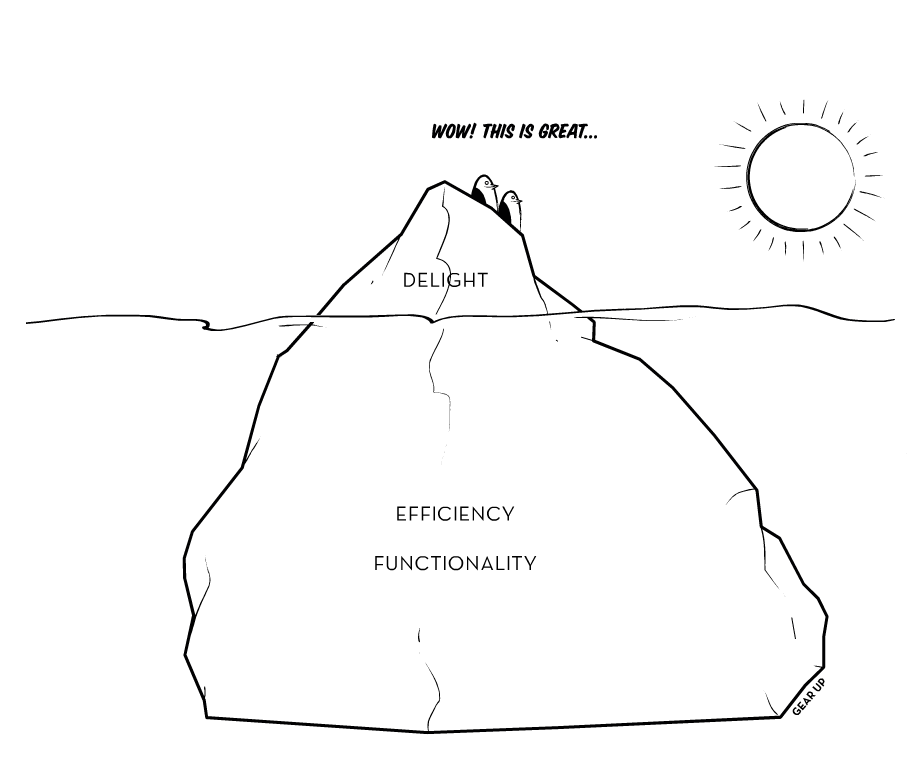
\includegraphics[width=0.7\textwidth]{images/delight}
	\caption{Iceberg of customer needs, \cite[p. 27]{Ramfelt}}
	\label{fig:DelightIceberg}
\end{figure}

%Another part of delight is about storytelling. This is about how customers tell a story about a product. The aim is, that this story is friction-free, which means, that the company and a customer tell a story that makes others to love the product. As soon as the story of a product is friction-free, the company created delight. There is no need of a lot of different unique innovations. Sometimes it is just one cool feature that creates enough delight.

\subsection{The core problem with delight}
Creating delight for the ChildFund Alliance proposal is important.  Therefore the target audience or in other words the customer has to be defined. The target audience for any project is the key element for success. Delight is only the tip of the iceberg. Providing efficiency and functionality within a product to a some person is hard, if you do not know who he is. Furthermore without knowing who the customer is, it is not possible to find out his pain. The customer's pain is where a solution is being created. 

Within the ChildFund Alliance proposal the vision of the target audience is not clearly defined, thus they are based on own assumptions. Nevertheless the pains are on the one side that it is harder to get people to give and on the other side these people do not know anything about the people who actually get help. The ChildFund Alliance's solution is to inform the sponsors who receives the money or help, but is this a delight or just functionality?

Separating delight from functionality is hard, but makes the difference, if a customer uses a product or loves it. Functionality and efficiency are two core concepts which the product must provide. Delighting customers is the tricky part. Just because the sponsors see what is actually happening with the money is no delight, because this is not new: This is just a feature. Also the Facebook integration must not be a delight for a customer, because this is a basic feature today. If the customer does not use Facebook, then there will be no delight at all. Regarding the customers there is always a different delight. Someone might benefit from a Facebook stream of information, others are just fine with a letter from a child. The problem that was mentioned in the beginning is still crucial: Who is the customer? If the ChildFund Alliance focuses on a Facebook integration, research should be done, if the sponsors really want to have that information on a social platform like this. Maybe the need for an own social platform regarding funding is needed.
	
\subsection{A solution to delight the customer}
To understand how it is possible to delight the customer the question must be answered, what the customer actually buys. Besides that he definitely does not buy any real goods, he invests the money to “feel better”: His self esteem raises and he feels satisfaction for helping. He might also buy himself into the giving community or just the status of being an investor in this domain. Some might also donate to alleviate his conscience, but a sponsor is just a simple human being, which means he gives and forgets.

One solution is therefore to inform a sponsor about what happens with the money. There are several attempts for creating delight for the customer. One example is that the customer can actually see the money chain, maybe also in real time on a website. Where is the money, for what was it used and so forth. Again the question is, if there are customers who would like to have that information on a website, which is browsable for anyone. A survey will help to find out, what features are really needed, and it could also give insights for a possible delight. The outcome of a survey might be, that sponsors would like to have an own portal to share the information or that they want to share that kind of information on Facebook. They could also make suggestions what they would like to have as a feature from the ChildFund Alliance. Listening to those people can create a delight for them, because they actually participate in building a tool. Another delight could be that the ChildFund Alliance is the most trustworthy foundation, because they have the lowest overhead costs. This delight automatically comes with a visible money chain. 

The different things that are produced or bought by the sponsor's money can also be a delight, e.g. a school building. There is no need that his face is on that, but just letting him know, that this school was build by his money. The look of the landscape changes and a town might look different than before. A small step aside to philosophy shows, that all the buildings or paintings make artists immortal. This might also happen to a sponsor, if his name is at least somewhere in the school building.

The customers should talk about the ChildFund Alliance without any friction, which is called friction-free story telling. They need to love the project to tell other possible customers — regarding to the sponsorship steam — only positive aspects of becoming a member. Creating a friction-free story with the suggestions made above is not achievable without asking actual customers. Do they believe the story? And do they tell the story someone else? This is the aim of creating delight and makes the marketing even easier, because the customers will also do it for you. They will have passion about how to donate money and how nice it is to see what actually happens with the money. If Facebook is used, they become fans, make suggestions and will tell other friends to donate.
